\begin{frame}
  \frametitle{\problemtitle}
  \begin{block}{Problem}
    Given an uppercase string, find all of its transformations into lowercase, where each \texttt{SS} may transform to either \texttt{ss} or \texttt{B} (approximating the German `ß'). The string contains at most three \texttt{S}.
  \end{block}
  \pause
  \begin{block}{Solution}
    \begin{itemize}
      \item<+-> If the string contains \texttt{SSS}, there are three solutions, replacing \texttt{SSS} with \texttt{sss}, \texttt{sB} and \texttt{Bs} respectively.
      \item<+-> Otherwise, if the string contains \texttt{SS}, there are exactly two solutions, one with \texttt{ss} and one with \texttt{B}.
      \item<+-> Otherwise, the only solution is the lowercase version of the string.
      \item<+-> Sample Implementation in Python:
        \vspace{3mm}

        \hspace{5mm}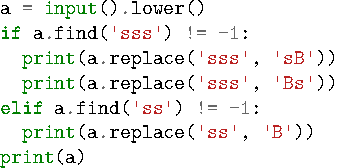
\includegraphics[width=0.4\textwidth]{python}
    \end{itemize}
  \end{block}
\end{frame}
